\documentclass[10pt,twocolumn]{article}
\usepackage[margin=0.75in,columnsep=0.28in]{geometry}
\usepackage{times}
\usepackage{amsmath}
\usepackage{graphicx}
\usepackage{booktabs}
\usepackage{array}
\usepackage{xcolor}
\usepackage{titlesec}
\usepackage{enumitem}
\usepackage[colorlinks=true,linkcolor=blue,citecolor=blue,urlcolor=blue]{hyperref}

\setlength{\parindent}{1em}
\setlength{\parskip}{0pt}

\renewcommand{\thesection}{\Roman{section}}
\renewcommand{\thesubsection}{\thesection-\Alph{subsection}}
\titleformat{\section}{\normalfont\large\bfseries}{\thesection.}{0.6em}{}
\titleformat{\subsection}{\normalfont\bfseries}{\Alph{subsection}.}{0.5em}{}
\titlespacing*{\section}{0pt}{8pt}{4pt}
\titlespacing*{\subsection}{0pt}{6pt}{3pt}

% Placeholder for work not yet done. grep for "\gap" before submitting;
% every one should be filled in or removed.
\newcommand{\gap}[1]{\par\noindent\colorbox{yellow!40}{\parbox{\dimexpr\linewidth-2\fboxsep}{\small\textbf{TO DO:} #1}}\par}

\begin{document}

\twocolumn[
\begin{center}
{\LARGE \bfseries Court Vision: Motion Planning for an \\ Obstacle-Aware Ball-Dribbling Mobile Robot \\[4pt]}
{\large RBE 550 Motion Planning --- Final Report \\[4pt]}
{\normalsize Rudy Arsenault, Tracy Yang \\
Worcester Polytechnic Institute \\[6pt]}
\end{center}
\vspace{4pt}
\hrule
\vspace{6pt}
{\small \noindent \textbf{Abstract}---We present a simulated mobile robot
that dribbles a ball with a paddle end-effector through a cluttered course,
choosing where each bounce lands so that the ball, the arm, and the
chassis all stay clear of obstacles. An offline planner searches over
position, heading, and \emph{time}, then over the arm angle along the
result, proving a run collision-free in advance when obstacle motion is
known; a schedule-tracking controller keeps the real run within 6.3\,cm of
that plan (0.6\,cm on average). Letting the planner choose where the ball
lands, rather than fixing it beside the chassis, solves 25 of 60 dense
courses against 7. A live planner handles obstacles that roam at their own
speeds, turn at random, and bounce off each other and the robot: it senses
them at every contact, predicts their bounces, routes with D*~Lite, and
picks each step with a dynamic-window local planner, finishing 27 of 30
roaming courses against 19 for D*~Lite alone and 9 for hybrid A*
replanned online. The robot slows in narrow passages, speeds up in the
open and when chased, and keeps the ball in bounds. Paddle contacts are
rigid-body impacts whose energy is fully accounted for.
\gap{Update the abstract with the Objective~5 evaluation and terrain
results.}}
\vspace{8pt}
\hrule
\vspace{10pt}
]

% =====================================================================
\section{Introduction}
A basketball player dribbling through a crowd solves two coupled
problems at once: where to send the ball next, and where to put their body
so they can meet it there. Our robot faces the same coupling. Its base
cannot simply steer around clutter, because it must be at the ball's next
contact point; when the nominal next bounce is blocked, the robot must
instead \emph{redirect} the ball to a reachable, collision-free spot and
plan the base to meet it. The proposal set five objectives: (1) a dribble
model, (2) a mobile base that dribbles while moving, (3) a static obstacle
course, (4) a redirect-the-bounce planner, and (5) an evaluation, with a
stretch goal of obstacles that move during a run.

Objectives~1--3 were complete at the Week~8 status update. This report
covers the redirect planner and its test against a no-redirect baseline
(Objective~4), its extension to obstacles moving on a known schedule and
then to obstacles whose motion must be sensed and predicted (the stretch
goal), an energy-consistent contact model, mobile-base limits, the success
criteria we hold the system to, and the evaluation to date (Objective~5).

% =====================================================================
\section{Background and Related Work}
\textbf{Dribbling.} Bühler, Koditschek, and Kindlmann formalized juggling
as an intermittent dynamical task and introduced the mirror law, a
feedback rule whose end-effector motion is a distorted reflection of the
ball's \cite{buehler1994}. Bätz et al.\ showed basketball dribbling shares
the same hybrid impact/flight dynamics and demonstrated it on a
stationary arm \cite{batz2009,batz2009icra}. DribbleBot moved dribbling
onto a walking quadruped over rough terrain, without discrete obstacles or
an explicit planning layer \cite{dribblebot2023}.

\textbf{Planning among obstacles.} Hybrid A* searches a lattice of short
kinematically feasible arcs over continuous position and heading
\cite{dolgov2010}; we extend its state with time. D*~Lite incrementally
repairs a shortest-path solution as edge costs change and the robot
moves, re-expanding only what the change invalidates \cite{koenig2002}.
The dynamic window approach selects velocities by forward-simulating
candidates and scoring progress against clearance \cite{fox1997}, and
velocity obstacles reason about collisions with moving obstacles in
velocity space \cite{fiorini1998}. Our live planner pairs a D*~Lite global
route with a dynamic-window local step, a standard global/local split.

% =====================================================================
\section{Success Criteria}
\label{sec:criteria}
Prompted by feedback on the status update, we fixed in advance what
counts as success, so results are judged against targets rather than
described after the fact. A live run \emph{finishes} only if the robot
crosses the finish line still dribbling; it otherwise ends the moment the
dribble does, as \emph{dribble lost} (the ball escaped the paddle),
\emph{out of bounds}, or \emph{timeout} (120\,s).
Table~\ref{tab:criteria} lists each criterion and where it stands;
Section~\ref{sec:results} has the evidence.

\begin{table}[h]
\centering
\small
\setlength{\tabcolsep}{3pt}
\begin{tabular}{@{}p{4.0cm}p{3.1cm}@{}}
\toprule
\textbf{Criterion} & \textbf{Result} \\
\midrule
Offline: zero collisions on every course it accepts & Met: 0 in 31 runs \\
Offline: ball within 5\,cm of its plan & Not met: 6.3\,cm worst, 0.6\,cm mean \\
Redirect solves more courses than no-redirect & Met: 25 vs.\ 7 of 60 \\
Live: $\ge$90\% of roaming courses finished & Met on the 30 shared courses (27); 77\% (46/60) on a wider set \\
Live: $\le$1 collision per run on average & Met: 0.43 (0.58 on 60) \\
Live: mean replan within one dribble cycle ($\approx$300\,ms) & Met: 119\,ms (worst 492\,ms) \\
Unexplained ball energy $<$1\% of paddle work & Met: 0.06\% mean \\
Paddle and base within actuator limits & Met by construction \\
Completion degrades gracefully with density & \textit{Pending (Obj.~5)} \\
\bottomrule
\end{tabular}
\caption{Success criteria and status.}
\label{tab:criteria}
\end{table}

% =====================================================================
\section{System Overview}
Everything runs in PyBullet at 240\,Hz. The ball is a dynamic sphere; the
chassis, arm, and paddle are kinematic bodies posed every step
(Fig.~\ref{fig:hero}). The paddle sits over the ball's real position and
the chassis one arm length ($0.5$\,m) away at the arm angle $\phi$, which
is also the chassis's yaw: chassis and arm turn together as one rigid
assembly. Each contact, the planner chooses where the ball lands next and
$\phi$.

\begin{figure}[t]
\centering
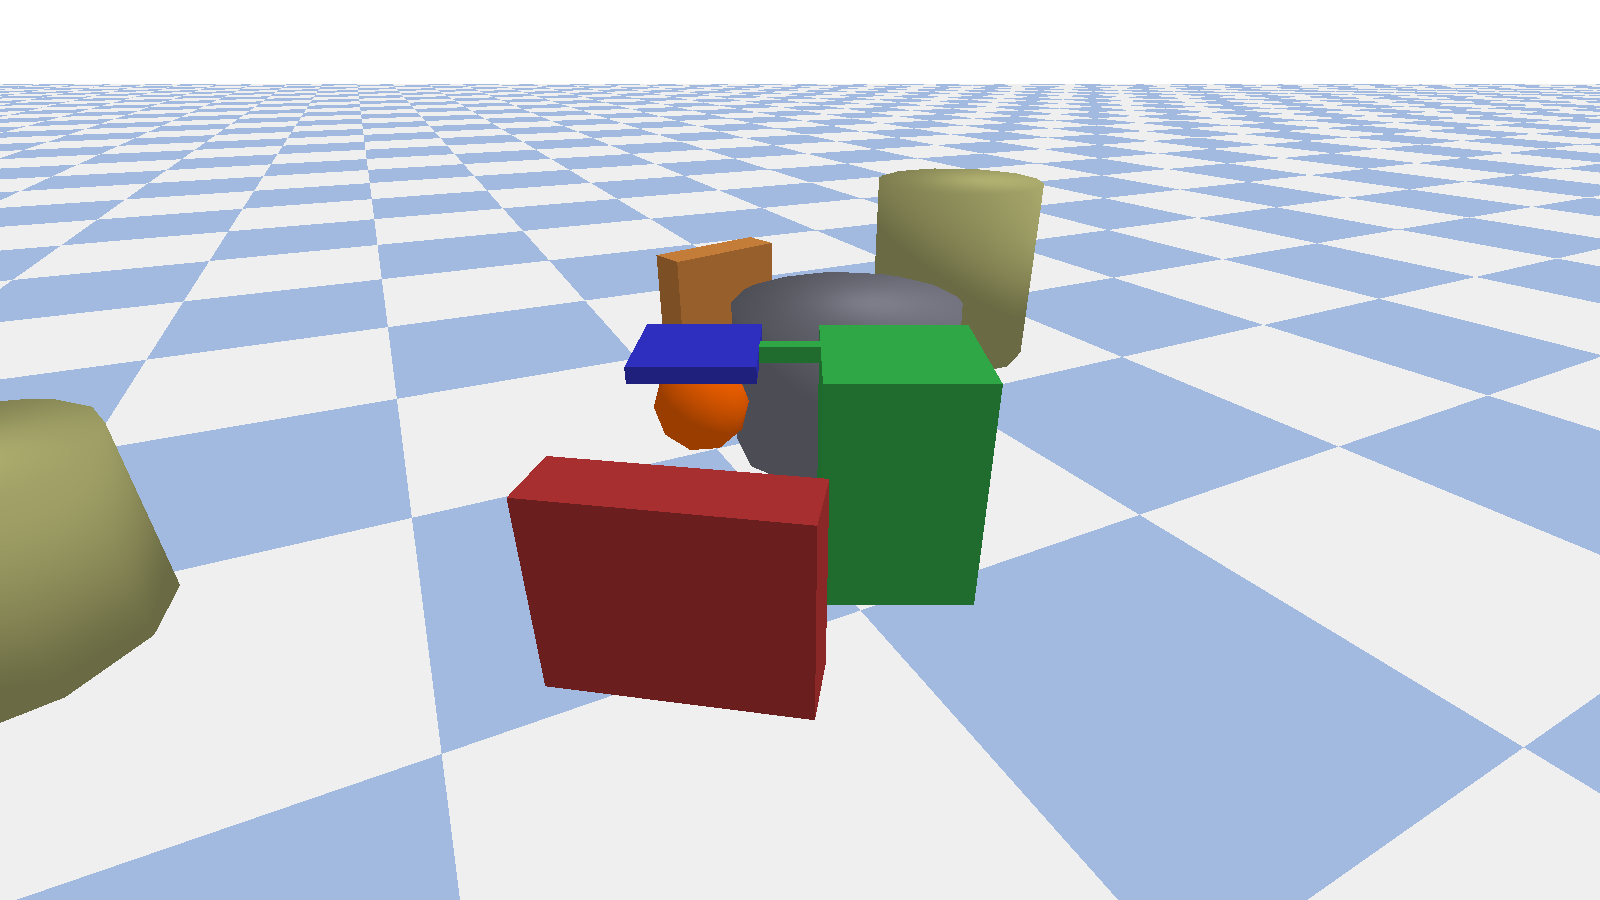
\includegraphics[width=\linewidth]{figures/hero.png}
\caption{The robot threading a gap: green chassis, arm, blue paddle over
the orange ball. Tinted obstacles are moving.}
\label{fig:hero}
\end{figure}

\textbf{Mobile-base limits.} The chassis may move at most 0.5\,m/s and
turn at most 90\,$^\circ$/s; because its yaw is $\phi$, the turn-rate
limit also caps how fast the arm angle can change. The ball's horizontal
speed is capped at 0.7\,m/s, leaving the arm room to move the ball
relative to a chassis already at cruise. Both planners enforce all three.

\textbf{Speed that follows the space.} The robot's cruising speed depends
on how much room it has: 0.15\,m/s with no free space between the chassis
and the nearest static obstacle, rising linearly to 0.45\,m/s at 0.5\,m or
more. Only static obstacles count. Narrow passages are fixed geometry,
and in our first version, slowing down near moving obstacles only gave
them longer to reach the robot (24 vs.\ 26 of 30 finishes).

\textbf{Courses (Objective~3).} Each course draws crates, pillars, and
walls of random size, position, and orientation for a $6\times3$\,m lane
(Fig.~\ref{fig:obstacles}), keeping each only if it is at least 0.4\,m
from every other obstacle's bounding circle. This gives 6.2 obstacles per
roaming course on average and 4.3 per oscillating course, since an
oscillating obstacle also reserves its whole sweep. About half the
obstacles move, in one of two ways:
\begin{itemize}[leftmargin=*,itemsep=1pt,topsep=2pt]
\item \emph{Oscillating} across the lane on a known sinusoid
(0.3--0.6\,m amplitude, 4--8\,s period).
\item \emph{Roaming}: each obstacle has its own base speed, drawn from
0.05--0.40\,m/s, so some crawl and some outrun the robot's cruise. It
turns at random moments (on average every 2.5\,s) by up to
$\pm120^\circ$, varying its speed by up to $\pm30\%$ of its base. It
bounces off the course edges, the static obstacles, each other, and the
robot's chassis, using the chassis's true shape.
\end{itemize}
Collisions between obstacles are detected before each step, so they never
overlap: over 100 roaming courses simulated for 300\,s (303 movers), the
closest two came was touching (0.002\,mm apart). Turns are drawn from the
course seed, so runs are reproducible, but no planner sees the turn
schedule.

\begin{figure}[t]
\centering
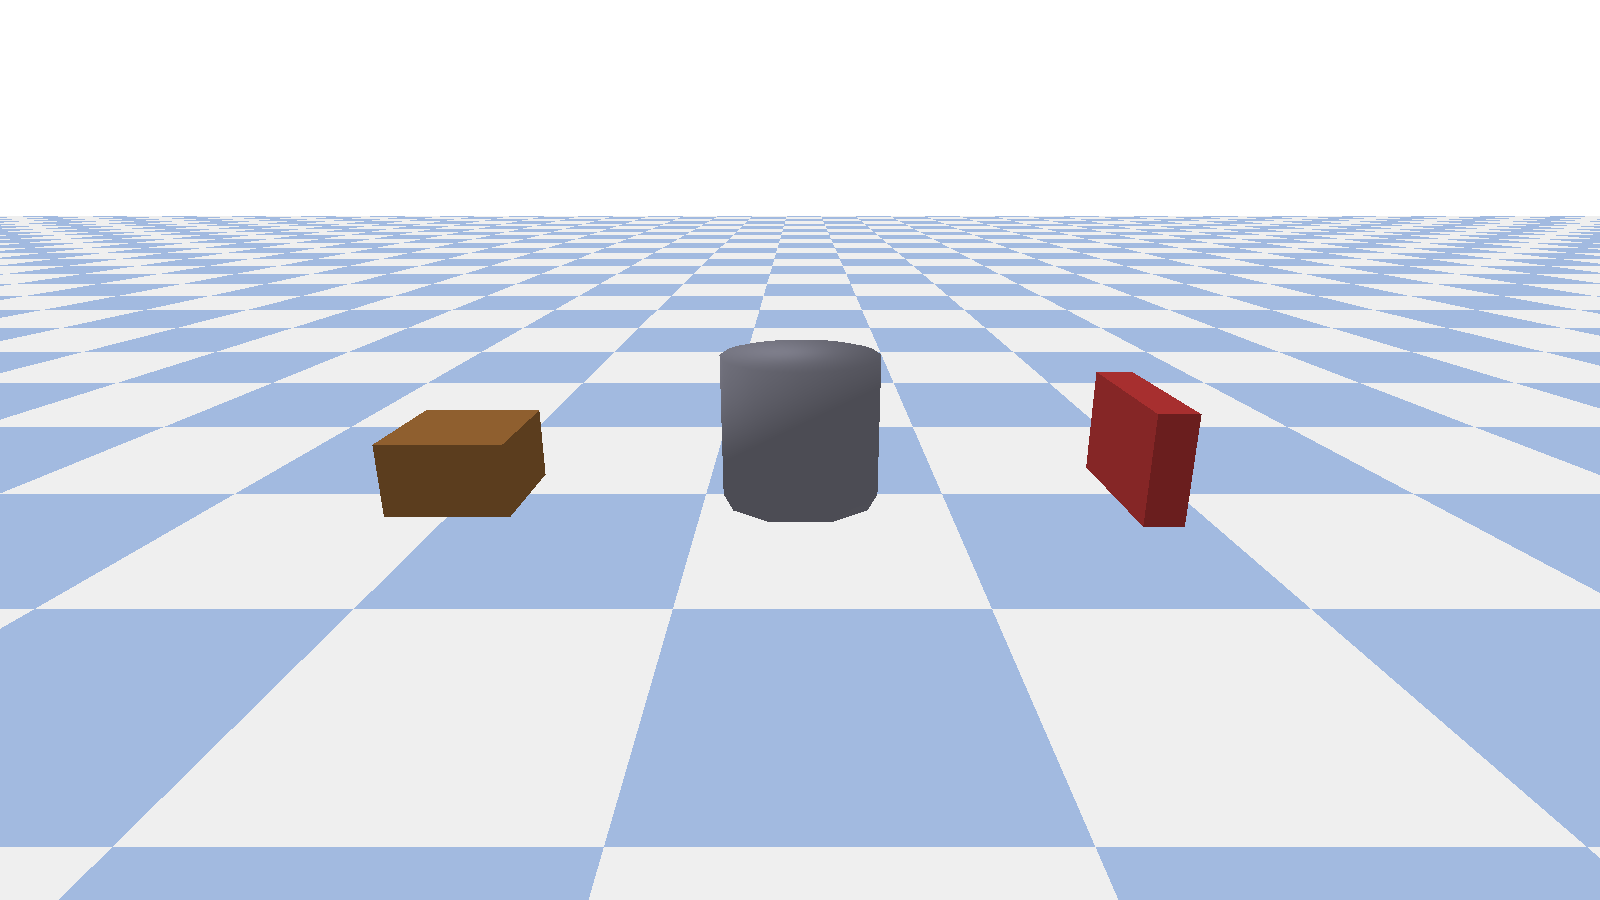
\includegraphics[width=\linewidth]{../figures/obstacle_types.png}
\caption{The three obstacle kinds and their size ranges.}
\label{fig:obstacles}
\end{figure}

% =====================================================================
\section{Dribble Model and Energy-Consistent Contact (Objective~1)}
\label{sec:energy}
Between contacts the ball is a free projectile, bouncing off the floor
with PyBullet's restitution model (coefficient 0.85). We removed
PyBullet's default linear damping (0.04\,s$^{-1}$), an unmodeled drag that
the planners' ballistic timing model does not include.

At each paddle contact, the vertical outgoing velocity follows the mirror
law: $-v_{\text{push}} = -2.2$\,m/s whatever the incoming speed, so the
bounce height stays constant \cite{buehler1994}. This gives 3.3 contacts
per second; we slowed it from 3.0\,m/s (4.3 per second) for a more
deliberate dribble, and much below 2\,m/s the ball would barely return to
the paddle. The horizontal outgoing velocity $\mathbf{v}_{xy}$ is the
planner's push. Earlier versions simply overwrote the ball's velocity,
with no impulse, no paddle work, and no account of where the added energy
came from. The contact is now a frictionless rigid-body impact between the
ball and a much heavier paddle. With incoming velocity $\mathbf{v}$,
desired outgoing velocity $\mathbf{v}'$, and $\Delta\mathbf{v} =
\mathbf{v}' - \mathbf{v}$, the impulse must lie along the face normal, so
the paddle face tilts to $\mathbf{n} = \Delta\mathbf{v}/\|\Delta\mathbf{v}\|$
and is driven at normal speed
\begin{equation}
u = \frac{\|\Delta\mathbf{v}\|}{1+e} + \mathbf{v}\cdot\mathbf{n},
\end{equation}
with paddle restitution $e = 0.8$. The paddle does work
$W = m\|\Delta\mathbf{v}\|\,u$, of which
$\tfrac12 m(1-e^2)(u - \mathbf{v}\cdot\mathbf{n})^2$ is lost in the impact and
the rest becomes the ball's kinetic energy. Tilting the face is literally
the proposal's ``alternate hit angle'' redirect; a 30\,$^\circ$ tilt limit and
3\,m/s paddle-speed limit bound the actuator.

Every run keeps an energy ledger: each step's change in the ball's
mechanical energy (translational, spin, and potential) is attributed to
paddle work and impact loss at contacts, floor loss while touching the
floor, and the integrator's known loss of $\tfrac12 m g^2 \Delta t^2$ per
step. What is left over is unexplained.

\gap{Optional: figure of the energy ledger over one run (paddle work vs.\
floor and impact losses).}

% =====================================================================
\section{Planning}

\subsection{Offline: Space--Time Hybrid A* with Known Obstacle Motion}
\label{sec:offline}
When every obstacle's future position is known, the whole run can be
planned and proven collision-free before it starts. The robot body's
center is searched over a lattice of $(x, y, \theta, t)$: each edge is a
0.1\,m forward arc at one of five turning rates, taking as long as the
cruising speed at that point allows, so the plan slows through narrow
gaps. Collision checks along each edge use each obstacle's position at
the interpolated time. A \emph{wait} edge holds the pose while dribbling
in place, offered only near moving obstacles and capped at 4\,s in total.
Each search is capped at 200{,}000 node expansions so a hopeless course
fails fast and is regenerated.

A second Dijkstra search over the found path picks $\phi$ at every point
from 23 candidates, verifying every \emph{transition} between consecutive
points with position, angle, and time interpolated together. Transitions
must respect the base speed, turn-rate, and ball speed limits, and each
moving obstacle is inflated by its peak speed times $\pm0.25$\,s, so a
small timing error cannot become a collision. Landing spots must stay
5\,cm inside the side lines and no more than 0.25\,m behind the start
line.

A plan proven at specific times holds only if the robot keeps to those
times. At each contact the controller aims the ball at where the plan
puts the paddle at the \emph{next} contact's time, pushing at whatever
speed covers that distance, and reads $\phi$ off the same clock.

\subsection{Redirect-the-Bounce and a No-Redirect Baseline (Objective~4)}
Because the arm-angle search chooses every landing point, redirection
happens by construction. To test whether it matters, we built the
baseline suggested in feedback on the status update: the same planner,
but with the ball rigidly fixed beside the chassis ($\phi = \theta \pm
90^\circ$, side chosen once per course). The ball's fixed position becomes
part of the robot's footprint in the body search, which also rejects any
turn the attached ball could not follow within the speed limits.

\subsection{Live: D*~Lite with a Dynamic-Window Local Step}
\label{sec:live}
Roaming obstacles turn at random and bounce off each other and the robot,
so their future is not known in advance. The live planner may only read
where each obstacle is \emph{now}, through a sensor that estimates velocity
from two readings 1/60\,s apart (a 60\,Hz camera), and replans at every
contact.

\textbf{Prediction.} At each contact, the planner rolls every obstacle
forward 2.5\,s from its sensed position and velocity under the obstacles'
own motion rule: straight lines, bouncing off the edges, the static
obstacles, and each other. This assumes the robot knows how obstacles
bounce, but not when they will turn. Without turns, it predicts 2\,s ahead
to within 0.3\,cm on average, where assuming constant velocity is off by
12\,cm (54\,cm in bad cases); with random turns, the 95th-percentile error
2\,s ahead is 41\,cm.

\textbf{Global route.} The lane is a $70\times31$ grid of 0.1\,m cells.
D*~Lite \cite{koenig2002} searches backward from every finish-line cell
over cells the robot body can occupy given the static obstacles. Moving
obstacles enter only as cost penalties along their predicted sweeps,
fading over 2.5\,s, so a passable course always has a route. When
penalties change between readings, only the affected vertices are
updated. Against plain Dijkstra on 8{,}000 random replans, D*~Lite
returned an optimal path every time.

\textbf{Local step.} A dynamic-window step \cite{fox1997} evaluates 33
body velocities (standing still, plus 16 directions at the cruising speed
and at an evasive 0.5\,m/s) by rolling each forward 2\,s against the
predicted obstacles. The cruising speed comes from the free space along
the next 0.6\,m of route. Velocities that reach a static obstacle within
0.4\,s, or a moving one within 1.0\,s, are discarded, as are moves that
would leave no in-bounds landing spot for the ball. The rest are scored
by progress toward a point 0.3\,m along the route (capped at the cruising
speed), clearance up to 0.5\,m, time to collision, and a cost for the
evasive speed. When an obstacle within 1.5\,m is behind the robot,
closing, and would reach it within 2\,s, the robot is \emph{chased} and
cruises at the evasive speed instead.

\textbf{Arm angle.} $\phi$ is chosen per contact from the same 23
candidates: within the turn-rate limit, with the landing point reachable
within the ball speed limit, 5\,cm inside the side lines, and clear of
every obstacle's predicted position along the ball's flight and for 1\,s
after. Of those, the one closest to the current angle wins, with a mild
preference for the ball beside the chassis and a penalty for landing
within 0.25\,m of a side line, so the arm starts steering the ball inward
before it can be trapped against the line. When no candidate is fully
clear, the fallback is the in-bounds spot with the most room from
obstacles and the side lines.

\subsection{Logging What Binds}
To answer whether obstacles or the base's speed limit the robot, both
planners record what constrained each decision. Offline: at each path
point, whether both nominal landing spots beside the chassis were blocked
by obstacles; at each transition, whether the turn-rate, base-speed, or
ball-speed limit was at least 95\% used. Live: at each contact, which
constraint ruled out the arm angle the robot would otherwise have
preferred, and whether the local step gave up progress to keep clear.

% =====================================================================
\section{Results}
\label{sec:results}
All runs are headless and deterministic for a given seed. Collisions are
ground truth: the real chassis and ball against every obstacle's real
position at the real time, with no planning margin.

\subsection{Offline Planner}
\label{sec:offline-results}
On the 10-course benchmark (\texttt{planner\_benchmark.py}, oscillating
obstacles), the planner needed 3.0 course generations on average (worst
8), took 15.3\,s (worst 49.8\,s), and produced paths 1.7--23.3\% longer
than the straight line (mean 7.3\%); 7--34\% of path points (mean 20\%)
were redirected away from the straight-ahead landing spot. Executing 20
offline plans with the schedule-tracking controller, all 20 finished with
\textbf{zero overlaps} with any obstacle, and the ball stayed within
0.6\,cm of its planned position on average. The worst deviation was
6.3\,cm, missing our 5\,cm target; it was 3.2\,cm before the plan's speed
varied with clearance, and the sharper speed changes between steps are the
likely cause. The 99th percentile stayed below 4.5\,cm on every course.
Before the controller tracked the plan's clock, runs fell 3--19\,s behind
schedule and 4 of 5 test courses collided with moving obstacles.

\subsection{Does Redirecting the Ball Matter?}
Table~\ref{tab:redirect} plans 60 raw courses (4.3 obstacles, 1.5 moving
on average) with and without redirection, and records at which stage each
failure occurred.

\begin{table}[h]
\centering
\small
\setlength{\tabcolsep}{4pt}
\begin{tabular}{@{}lrrr@{}}
\toprule
& \textbf{Solved} & \textbf{No body path} & \textbf{No arm seq.} \\
\midrule
With redirect    & 25 & 24 & 11 \\
No redirect      & 7  & 53 & 0 \\
\bottomrule
\end{tabular}
\caption{Objective~4 ablation on 60 raw courses. ``No arm seq.'': a robot
body path exists but no arm-angle sequence along it.}
\label{tab:redirect}
\end{table}

Redirection more than triples the courses solved: 18 are solved only with
it and none only without, and where both succeed the paths are the same
length (6.31 vs.\ 6.30\,m). Most failures are the body search finding no
route at all. But 11 of the full planner's failures found a body path with
no workable arm sequence along it: the full planner's body search ignores
the arm, so it can commit to a route the arm cannot follow.

\subsection{What Binds: Obstacles or the Base?}
\label{sec:binding}
Across the 11 oracle plans on roaming courses, both nominal landing spots
were blocked by obstacles at 27\% of path points, while the base turn-rate
and speed limits were never binding and the ball speed limit bound on
0.4\% of transitions. Live, obstacles ruled out the preferred arm angle at
10\% of contacts and the side lines at 4\%; the ball-speed limit did so at
3\% and the turn-rate limit at 0.1\%. The local step gave up progress to
keep clear at 34\% of contacts, backed away from the route at 3\%, and ran
from a chasing obstacle at 3\%. At these limits (0.5\,m/s, 90\,$^\circ$/s),
the bottleneck is where the ball can land among the obstacles, not how fast
the base can get there.

\subsection{Live Planners Compared}
Table~\ref{tab:planners} compares the live planners on the same 30 roaming
courses (6.2 obstacles, 3.2 moving). Only the search changes; sensing,
prediction, the arm-angle choice, and the controller are shared. Live
hybrid A* reruns the offline space--time search from scratch at each
contact against the predictions. The oracle row is the offline planner
given the obstacles' true future motion on the same courses.

\begin{table}[h]
\centering
\small
\setlength{\tabcolsep}{2.5pt}
\begin{tabular}{@{}lrrrrr@{}}
\toprule
\textbf{Planner} & \textbf{Done} & \textbf{Coll.} & \textbf{Time} & \textbf{Over.} & \textbf{Replan (ms)} \\
\midrule
D*~Lite + DWA    & 27/30 & 13 & 32.8 & 52\% & 119 / 492 \\
D*~Lite alone    & 19/30 & 19 & 43.3 & 35\% & 85 / 327 \\
Hybrid A* (live) & 9/30  & 29 & 71.3 & 19\% & 5635 / 24419 \\
\midrule
Oracle           & 11/30 & 0  & 22.3 & 5\%  & --- \\
\bottomrule
\end{tabular}
\caption{Live planners on 30 shared roaming courses. Done: finished
while still dribbling. Coll.: distinct collisions summed over all runs.
Time: mean seconds over finished runs. Over.: median path length beyond
the 6\,m straight line. Replan: mean / worst per contact. The oracle
found no plan for 19 courses; it never collided on the 11 it planned.}
\label{tab:planners}
\end{table}

D*~Lite + DWA finished the most courses, fastest, with the fewest
collisions; its three failures were one lost dribble and two balls knocked
out of bounds after an obstacle hit them. D*~Lite alone timed out on 3
courses and lost the ball on 8, 5 of them out of bounds. The price of the local step is path
length: rather than standing still while waiting for a gap, it keeps
stepping to stay clear of approaching obstacles, so its median path is
52\% longer than the straight line. Live hybrid A* needed 5.6\,s per replan
on average against a 300\,ms dribble cycle; the simulation does not charge
planning time, so its numbers flatter it, and half its runs timed out. The
oracle never collides but plans only 11 of 30 courses: its forward-only
motion, time margin, and search budget make it far more conservative than
the live planners, so it bounds safety, not completion.

\subsection{Tuning the Live Planner}
Each change below was kept only if it held up on the same set of courses.
\begin{itemize}[leftmargin=*,itemsep=1pt,topsep=2pt]
\item \textbf{Giving way earlier.} Rejecting velocities that collide within
1.0\,s (was 0.6\,s) and valuing clearance up to 0.5\,m at double weight
raised finishes from 25 to 28 of 30 and cut collisions from 47 to 27 on
an earlier version of the courses.
Making backing up cheaper did no better: stepping aside or waiting is
usually the better escape.
\item \textbf{Speed from clearance.} With the slower dribble, a fixed
0.25\,m/s finished 26 of 30 with 25 collisions in 12 runs; speed from
clearance finished 25 with 21 collisions in only 7 runs.
\item \textbf{Running when chased.} On 90 courses, the chase speed-up cost
5 finishes when the top cruise was 0.35\,m/s: the robot could not
outrun its pursuer. With 0.45\,m/s in the open it added 2 finishes, cut
collisions by about a quarter, and brought the median run from 37 to
33\,s, so we kept both.
\item \textbf{Predicting bounces.} On 90 courses without random turns,
bounce-aware prediction finished 75 against 72 for constant velocity, and
adding the longer look-ahead (2\,s local, 2.5\,s route, 1\,s past each
landing) reached 76 with 37 collisions instead of 50. With constant-velocity
prediction, looking further ahead had made things worse.
\item \textbf{Uncertainty margins backfired.} Widening each predicted
obstacle in proportion to how far ahead it was predicted, every variant
finished fewer courses (50--70 of 90 against 72): the wider keep-out zones
pushed the robot toward the side lines, where it lost the ball out of
bounds. They are off.
\item \textbf{Shielding the ball} with the chassis from the nearest moving
obstacle was mixed ($+2$ finishes at one speed, $-4$ at another) and is
off.
\end{itemize}

\subsection{Keeping the Ball in Bounds}
Watching runs showed the arm itself sometimes bouncing the ball out: driving
along a side line with the ball on the outside, the turn-rate limit kept
the arm from swinging it back inward in time, and the fallback for that
case ignored the boundary. In a 30-run check, 14 runs aimed at least one
bounce outside the court. With in-bounds landing spots and fallback, moves
filtered by whether the ball can stay in, the 5\,cm margin, and the
side-line penalty (Section~\ref{sec:live}), none did. At the same time we
began ending each run when the dribble ends: previously the robot was
placed beside the ball even after the dribble was lost, so a ball rolling
over the finish line counted. On 90 courses, the old count of 84 finishes
fell to 77 with the bounds fixes and to 71 under honest counting.

\subsection{Robustness to Unpredictable Obstacles}
Table~\ref{tab:robust} runs D*~Lite + DWA on 60 roaming courses with the
obstacles' random turns off and on, using bounce-aware or constant-velocity
prediction. With turns on, the planner's model of the obstacles is wrong
every few seconds.

\begin{table}[h]
\centering
\small
\setlength{\tabcolsep}{2.5pt}
\begin{tabular}{@{}llrrrrr@{}}
\toprule
\textbf{Turns} & \textbf{Predict} & \textbf{Done} & \textbf{Coll.} & \textbf{OOB} & \textbf{Lost} & \textbf{Time} \\
\midrule
Off & Bounce   & 45/60 & 43 & 5 & 8  & 37.0 \\
On  & Bounce   & 46/60 & 35 & 5 & 8  & 33.9 \\
Off & Constant & 42/60 & 54 & 5 & 11 & 35.2 \\
On  & Constant & 45/60 & 38 & 7 & 7  & 35.9 \\
\bottomrule
\end{tabular}
\caption{Robustness on 60 roaming courses (6.2 obstacles, 3.1 moving).
OOB: ball out of bounds. Lost: dribble lost. The rest of the failures are
timeouts.}
\label{tab:robust}
\end{table}

Random turns do not hurt: completion is within one course with or without
them, for either predictor. Bounce-aware prediction finishes as many or
more courses with fewer collisions in both settings, most clearly without
turns (54 to 43 collisions), where its model is exact. Seeds 30--59 are
harder than the 30 shared courses of Table~\ref{tab:planners}: the default
finishes 19 of them, against 27 of the first 30. Of its 14 failures, 11
began with an obstacle hitting the ball; the other two balls out of bounds
were the arm's, and one run timed out.

\subsection{Energy Consistency}
Over 341 live runs, the ledger left on average 0.06\% of paddle work
unexplained. In the 283 runs where no obstacle struck the ball it closed
exactly (to $10^{-14}$); the remainder, at most 1.8\%, is energy exchanged
in ball--obstacle collisions. In a typical finished run the paddle did
143\,J of work; the floor took 121\,J, impacts 19\,J, and the integrator
4\,J. Paddle demands stayed modest: at most a 23.9\,$^\circ$ face tilt and
1.18\,m/s, and no contact ever hit the tilt limit.

\subsection{Comparison with an Obstacle-Free Baseline (Objective~5)}
\gap{Run \texttt{python experiments.py density}: completion, collisions,
path overhead, and redirect frequency vs.\ obstacle count (0, 2, 4, 6, 8),
the 0-obstacle row being the obstacle-free baseline, for D*~Lite + DWA and
the oracle. Add a figure of completion and collisions vs.\ density.}

\subsection{Terrain Variation}
\gap{Planned work (Rudy): dribbling up and down slopes, then over varied
terrain. Describe the approach and results once implemented. On a slope
the floor's tilted normal pushes the ball downhill at every bounce and
changes bounce timing, so the controller's ballistic model and the paddle
aim must account for terrain height and slope.}

\subsection{Demonstration}
\gap{Record and link demo videos (\texttt{--video}): an offline run with
oscillating obstacles and a live run with roaming obstacles.}

\begin{figure}[t]
\centering
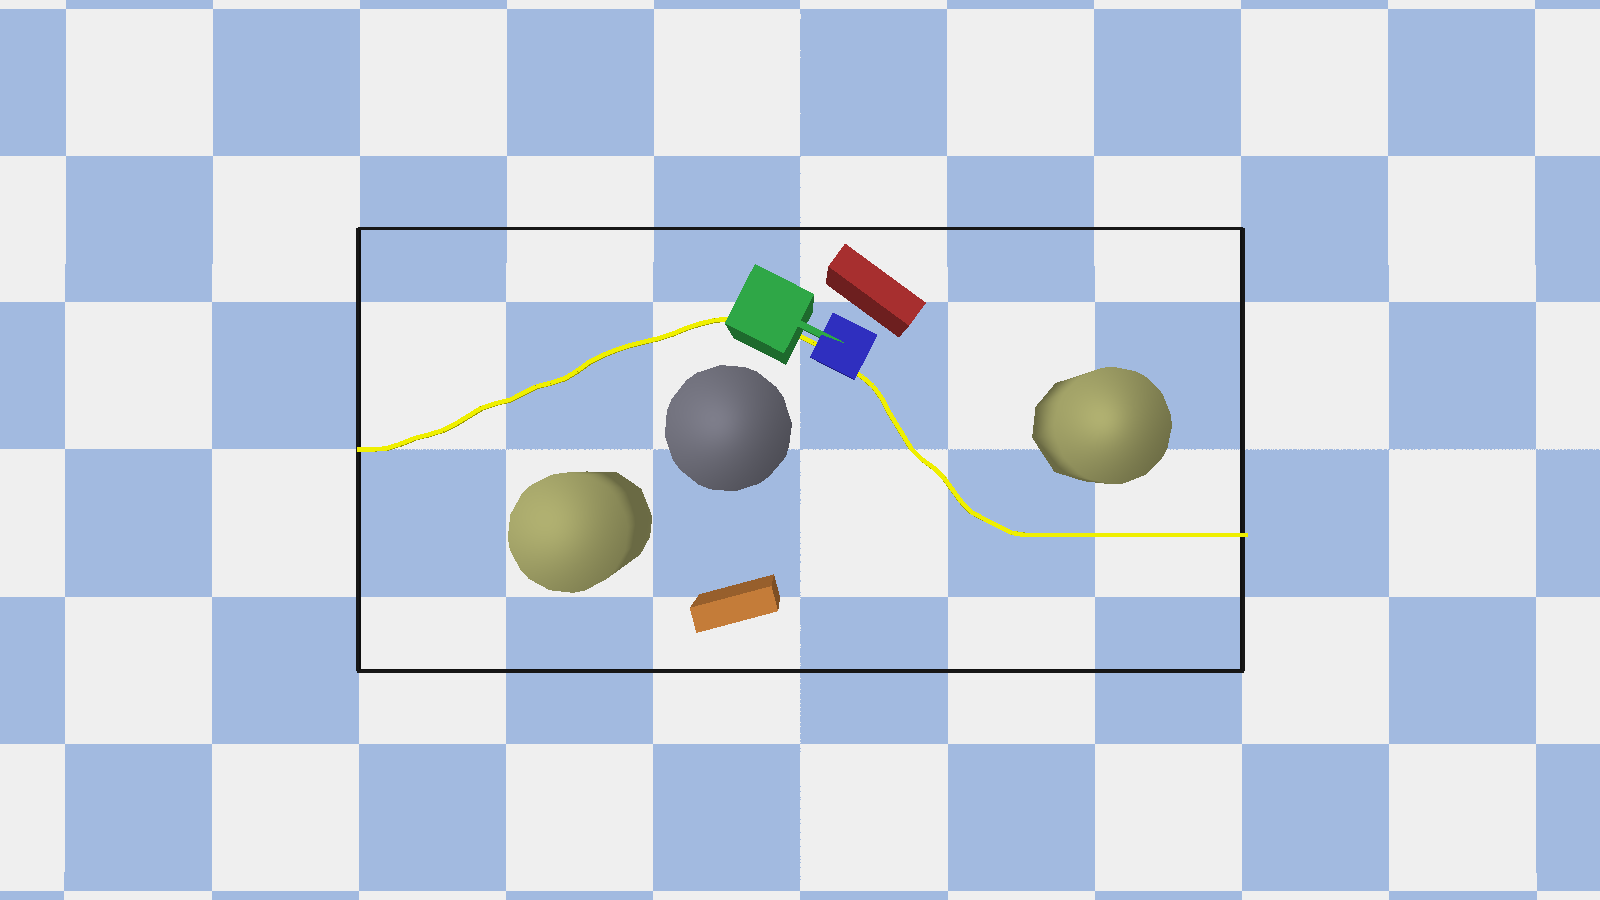
\includegraphics[width=\linewidth]{figures/overhead.png}
\caption{Overhead view of a roaming course with the oracle's planned
robot-body path (yellow) and the robot at 45\% of the way through.}
\label{fig:overhead}
\end{figure}

% =====================================================================
\section{Implementation and Running the Code}
Code is pure Python (NumPy, PyBullet).
\gap{Add the repository link and a README with setup steps.}

\begin{table}[h]
\centering
\small
\setlength{\tabcolsep}{3pt}
\begin{tabular}{@{}>{\ttfamily}l p{4.4cm}@{}}
\toprule
\textrm{\textbf{File}} & \textbf{Contents} \\
\midrule
simulation.py & Entry point; dribble loop, controllers, energy ledger, metrics \\
planning.py & Space--time hybrid A*, arm-angle search, no-redirect baseline \\
live\_planning.py & Sensor, prediction, D*~Lite + DWA, live hybrid A* \\
dstar\_lite.py & D*~Lite on an 8-connected grid \\
obstacles.py & Course generation, roaming motion, collision tests \\
physics.py & Ballistic timing, energy-consistent paddle impact \\
robot.py & Chassis, arm, paddle \\
evaluation.py & Redirect events, binding-constraint analysis \\
experiments.py & Batch experiments behind every results table \\
planner\_benchmark.py & Offline planner benchmark \\
render\_scene.py & Report figures \\
config.py & Shared constants and limits \\
\bottomrule
\end{tabular}
\caption{Source files.}
\label{tab:files}
\end{table}

\noindent Typical commands:
{\small
\begin{verbatim}
python simulation.py --seed 4
python simulation.py --planner offline
python simulation.py --speed 1 --video r.mp4
python experiments.py planners
python experiments.py redirect
python experiments.py robustness
\end{verbatim}}
\texttt{--planner} selects \texttt{dwa} (default), \texttt{dstar},
\texttt{hybrid}, \texttt{offline}, or \texttt{oracle} (the offline planner
on the live planners' course); \texttt{--motion} selects oscillating or
roaming obstacles; \texttt{--speed} sets GUI playback as a multiple of real
time (default 3, 0 for unpaced); \texttt{--headless} runs without a window.
Solved courses are cached on disk per seed, keyed on the planner, obstacle,
and configuration source. \texttt{experiments.py} writes raw rows to
\texttt{results/}.

% =====================================================================
\section{Responding to Status-Update Feedback}
\textbf{No-redirect baseline} (Raghu Vadlamani): using our own planner with
redirection disabled as the baseline directly tests the coupling
hypothesis (Table~\ref{tab:redirect}).

\textbf{Backtracking when the arm search fails} (Imaan Haider): on the
original sparse courses no failures were of this kind, but on dense ones
11 of 60 are, so retrying another body path is now worthwhile future work.

\textbf{What counts as ``good enough''} (Megan Carlson):
Section~\ref{sec:criteria}, including what counts as a finish.

\textbf{Is the bottleneck landing spots or base speed?} (Thomas DeSilva):
we added base speed and turn-rate limits and logged what binds; at these
limits it is obstacles (Section~\ref{sec:binding}).

\textbf{Source of failures, and drift from the assumed bounce} (Won Jun
Lee): failures are broken down by stage in Table~\ref{tab:redirect} and by
outcome in Table~\ref{tab:robust}. The drift question pointed at a real
problem: the robot fell up to 19\,s behind its plan, fixed by tracking the
plan's clock (Section~\ref{sec:offline-results}).

\textbf{Dynamic obstacles such as another person} (Sameer Augustine): the
live planner (Section~\ref{sec:live}), now with obstacles that turn
unpredictably, move at different speeds, and react to the robot.

\textbf{Energy consistency of the mirror law} (Prof.\ Flickinger): the
contact is now a rigid-body impact with full energy accounting
(Section~\ref{sec:energy}).

% =====================================================================
\section{Adaptability: Challenges and How We Adapted}
\textbf{Reactive $\rightarrow$ proven-in-advance arm planning}
(status update). A live arm-angle controller could only check that some
angle was clear at a point, never that the arm could get from one safe
angle to the next, so we replaced it with the transition-verifying search.

\textbf{Ball-centric $\rightarrow$ body-centric planning} (status
update). The chassis has the larger footprint, so the search plans its
center directly and derives the ball's path from it.

\textbf{A proof is only as good as its timing.} Adding time to the
search made plans collision-free on paper, but replaying real positions
against real obstacle positions found 4 of 5 courses colliding: the old
waypoint follower tracked \emph{where} the ball was but never \emph{when}.
We moved the controller onto the plan's clock, started the ball where the
plan starts it, and added speed limits and a time margin; collisions went
to zero. Measuring against ground truth, not the planner's own model, is
what exposed the gap.

\textbf{Known schedule $\rightarrow$ live replanning.} Roaming obstacles
break the offline planner's assumption that the future is known. Rather
than stretch the offline guarantee, we built a live planner that only
senses the present and kept the offline planner as an oracle, accepting
that collisions become a measured outcome rather than a guaranteed zero.

\textbf{Choosing the live algorithm by measurement.} D*~Lite alone
\cite{koenig2002} hard-blocked every cell an obstacle might soon reach,
which closed off the lane on dense courses and left the robot standing
still while obstacles ran into it. Moving the dynamic reasoning into a
dynamic-window step \cite{fox1997} worked better; replanning the offline
hybrid A* \cite{dolgov2010} live did worse and was too slow. We kept
D*~Lite + DWA.

\textbf{Making the obstacles harder on purpose.} Once bounce-aware
prediction made obstacles nearly perfectly predictable, a high completion
rate no longer showed the planner was robust. We gave obstacles random
turns and individual speeds and let them push off the robot, then measured
how much the planner degraded (Table~\ref{tab:robust}). Speeds had earlier
been capped at the robot's pace because fast obstacles caught the ball
from behind; we lifted the cap for variety and answered it with the chase
speed-up instead.

\textbf{Our own claims needed checking.} Answering feedback, we found the
status update's ``6--9 obstacles'' partly counted obstacles the generator
had placed inside one another when they did not fit; we fixed the
generator and relaxed the spacing to reach about 6 real obstacles. Our
no-redirect baseline twice solved 0 of 60 courses, a result that looked
decisive but was a bug both times: first the body search chose turns a
rigidly attached ball could not follow, then a start-line rule rejected the
very first pose because part of its arm-angle window sampled the ball a
few centimetres behind the line. Fixed, it solves 7. The energy ledger
initially left 8\% of paddle work unexplained, traced to PyBullet's
default drag. Counting a finish whenever the robot crossed the line
overstated our results by 6 of 90 courses.

\textbf{Intuitive fixes that failed.} Slowing near moving obstacles and
widening predicted obstacles for uncertainty both sound safer, and both
made things worse: the first gave obstacles more time to arrive, the
second crowded the robot against the side lines. We only learned this by
measuring each change against the same courses.

\textbf{Bugs found by testing against references.} D*~Lite occasionally
returned a slightly longer path; comparing against Dijkstra traced this to
floating-point ties between keys ending the search one expansion early.
Some courses never finished even with no moving obstacles: a robot at
$x = 5.96$\,m rounded into a goal cell centered on 6.0\,m and stopped
4\,cm short.

\textbf{Simulation speed.} The GUI ran at about a tenth of real time.
Profiling showed 41 of 46\,s spent in PyBullet debug-line calls, each
waiting about 20\,ms on WSL's software renderer; drawing the arm as a real
body and the route as one batched point set brought runs to several times
real time.

\gap{Add any further challenges from the remaining weeks, including
terrain.}

% =====================================================================
\section{Limitations and Future Work}
The live planner offers no safety guarantee: an obstacle that turns
unpredictably can still reach the ball, and nearly every remaining failure
starts that way. Recovering a knocked ball, rather than ending the run
when the dribble is lost, is the most direct route to more finishes.
Prediction assumes the robot knows how obstacles bounce, and the
simulation does not charge planning time. The live planner's active
avoidance lengthens paths; a smoothness term in the local step did not
help, and better waiting behavior is open. The offline body search ignores
the arm, which costs 11 of 60 dense courses; backtracking to a different
body path when the arm search fails is the natural fix. The offline
planner cannot reverse, and its tracking now misses the 5\,cm target by
1.3\,cm at worst.

\gap{Stretch goal 2 (multi-bounce lookahead): done or not, and what was
learned.}

\gap{Stretch goal 3: physical-feasibility discussion (sensing, paddle
actuator bandwidth, ball tracking). The paddle tilt and speed reported in
Section~\ref{sec:results} are a starting point.}

% =====================================================================
\section{Conclusion}
\gap{Write once the final evaluation is in.}

% =====================================================================
\section*{Appendix: Individual Contributions}
\subsection*{Rudy Arsenault}
\gap{Contributions since the status update (see the status report for
earlier work), including terrain variation.}

\subsection*{Tracy Yang}
\gap{Contributions since the status update (see the status report for
earlier work).}

\begin{thebibliography}{9}
\bibitem{buehler1994} M.~Bühler, D.~E. Koditschek, and P.~J. Kindlmann,
``Planning and control of robotic juggling and catching tasks,''
\emph{The International Journal of Robotics Research}, vol.~13, no.~2,
pp.~101--118, 1994.

\bibitem{batz2009} G.~Bätz, M.~Sobotka, D.~Wollherr, and M.~Buss, ``Robot
basketball: Ball dribbling -- a modified juggling task,'' in \emph{Advances
in Robotics Research}, T.~Kröger and F.~M. Wahl, Eds. Berlin, Heidelberg:
Springer, 2009, pp.~323--334.

\bibitem{batz2009icra} G.~Bätz, K.-K. Lee, D.~Wollherr, and M.~Buss, ``Robot
basketball: A comparison of ball dribbling with visual and force/torque
feedback,'' in \emph{Proc.\ IEEE Int.\ Conf.\ on Robotics and Automation
(ICRA)}, 2009.

\bibitem{dribblebot2023} Y.~Ji, G.~B. Margolis, and P.~Agrawal, ``DribbleBot:
Dynamic legged manipulation in the wild,'' in \emph{Proc.\ IEEE Int.\ Conf.\
on Robotics and Automation (ICRA)}, 2023.

\bibitem{dolgov2010} D.~Dolgov, S.~Thrun, M.~Montemerlo, and J.~Diebel,
``Path planning for autonomous vehicles in unknown semi-structured
environments,'' \emph{The International Journal of Robotics Research},
vol.~29, no.~5, pp.~485--501, 2010.

\bibitem{koenig2002} S.~Koenig and M.~Likhachev, ``D* Lite,'' in
\emph{Proc.\ AAAI Conf.\ on Artificial Intelligence}, 2002, pp.~476--483.

\bibitem{fox1997} D.~Fox, W.~Burgard, and S.~Thrun, ``The dynamic window
approach to collision avoidance,'' \emph{IEEE Robotics \& Automation
Magazine}, vol.~4, no.~1, pp.~23--33, 1997.

\bibitem{fiorini1998} P.~Fiorini and Z.~Shiller, ``Motion planning in
dynamic environments using velocity obstacles,'' \emph{The International
Journal of Robotics Research}, vol.~17, no.~7, pp.~760--772, 1998.
\end{thebibliography}

\end{document}
